\documentclass[conference]{IEEEtran}
\IEEEoverridecommandlockouts
% The preceding line is only needed to identify funding in the first footnote. If that is unneeded, please comment it out.
\usepackage{cite}
\usepackage{amsmath,amssymb,amsfonts}
\usepackage{algorithmic}
\usepackage{graphicx}
\usepackage{textcomp}
\usepackage{xcolor}
\def\BibTeX{{\rm B\kern-.05em{\sc i\kern-.025em b}\kern-.08em
    T\kern-.1667em\lower.7ex\hbox{E}\kern-.125emX}}


%coming from agere:
\usepackage{mathpartir} %mathpar
\usepackage{enumerate}
\usepackage[export]{adjustbox} %fbox around figures
\usepackage{changepage} %fbox around figures
\usepackage{caption}
\usepackage{subcaption}
\usepackage{fancyvrb}
        
\usepackage{verbatim}
%\newcommand{\sepehrsays}[1]{{\small\textbf{\textit{\color{blue}(*#1 -- Sep*)}}}}

\usepackage[belowskip=-13pt,aboveskip=0pt]{caption}

\usepackage[font=small,skip=0pt]{caption}



\begin{document}


\newtheorem{notation}{\textit{Notation}}[section]
\newtheorem{definition}{Definition}[section]
%\newtheorem{theorem}{Theorem}[section]
%\newtheorem{corollary}{Corollary}[section]
%\newtheorem{lemma}{Lemma}[section]
%\newtheorem{conject}{Conjecture}[section]
%\newtheorem{example}{Example}[section]
%\newenvironment{proof}[1]{\noindent\textit{Proof.}\ #1}{\qed\medskip}
% comments
\newcommand{\sepehrsays}[1]{{\small\textbf{\textit{\color{blue}(*#1 -- Sep*)}}}}

%basic semantics
\newcommand{\trace}{\tau}
\newcommand{\config}{\ensuremath{\kappa}}
\newcommand{\configs}{\mathcal{K}}
\newcommand{\traces}{\mathcal{T}}
\newcommand{\maptoinfo}[1]{\lfloor #1 \rfloor}
\newcommand{\ls}{\mathit{LS}}
\newcommand{\alog}{\mathbb{L}}
\newcommand{\alogs}{\mathcal{L}}
\newcommand{\configlog}{\ensuremath{\mathit{logof}}}
\newcommand{\tracelog}[2]{#1 \rightsquigarrow #2}
\newcommand{\sysid}{\mathbf{\mathfrak{s}}}
\newcommand{\rewrite}{\mathcal{I}}
\newcommand{\tracesim}{\colonapprox}
\newcommand{\simlogs}{\mathit{simlogs}}
\newcommand{\trprefix}{\mathit{prefix}}

%info algebra
\newcommand{\infoset}{\Phi}
\newcommand{\classes}{\Psi}
\newcommand{\comb}[2]{#1 \otimes #2}
\newcommand{\focus}[2]{{#1}^{\Rightarrow #2}}
\newcommand{\leqinfo}{\preccurlyeq}


%logic
\newcommand{\closure}{\mathit{Closure}}
\newcommand{\phifol}{\Phi_{\mathit{FOL}}}
\newcommand{\predsyms}{\mathit{Preds}}
\newcommand{\langfol}[1]{\mathit{FOL}({#1})}
\newcommand{\psifol}{\Psi_{\mathit{FOL}}}
\newcommand{\toFOL}[1]{\ensuremath{\mathit{toFOL}(#1)}}
\newcommand{\spec}{\mathit{spec}}
\newcommand{\callpols}{{\mathcal{LS}_{\mathit{call}}}}
\newcommand{\folp}[1]{\mathrm{#1}}
\newcommand{\triggers}{\mathit{Triggers}}
\newcommand{\logevent}{\mathit{Logevent}}
\newcommand{\guidelines}{\Gamma_G}



%pi
\newcommand{\srclang}{\Pi}
\newcommand{\trglang}{\Pi_{\mathrm{log}}}
\newcommand{\names}{\mathcal{N}}
\newcommand{\prefix}{\alpha}
\newcommand{\inprefix}[2]{#1(#2)}
\newcommand{\outprefix}[2]{\bar{#1}#2}
%\newcommand{\silprefix}{\tau}
\newcommand{\agents}{\mathcal{A}}
\newcommand{\topagents}{\mathcal{A}_\mathcal{U}}
\newcommand{\locagents}{\mathcal{A}_\mathcal{L}}
\newcommand{\nilproc}{\textbf{0}}
%\newcommand{\ifproc}[3]{\texttt{if~} #1 = #2 \texttt{~then~} #3}
%\newcommand{\ifnproc}[3]{\texttt{if~} #1 \neq #2 \texttt{~then~} #3}
\newcommand{\newproc}[2]{(\nu #1)#2}
%\newcommand{\procs}{\mathcal{P}}
\newcommand{\codebaseu}{\mathcal{C}_\mathcal{U}}
\newcommand{\codebasel}{\mathcal{C}_\mathcal{L}}
\newcommand{\bn}[1]{\mathit{bn}(#1)}
\newcommand{\fn}[1]{\mathit{fn}(#1)}
\newcommand{\subst}{\sigma}
\newcommand{\cntxt}{\mathcal{E}}
\newcommand{\congr}{\equiv}
\newcommand{\boundout}[2]{\bar{#1}\nu#2}
%\newcommand{\action}{\prefix}
%%\newcommand{\redx}[1]{\xrightarrow{#1}} % for labeled reduction
\newcommand{\redx}{\longrightarrow} % for unlabeled reduction
\newcommand{\callev}{\mathsf{callEvent}}
\newcommand{\emitev}{\mathsf{emit}}
\newcommand{\addprecond}{\mathsf{addPrecond}}
\newcommand{\sendprecond}{\mathsf{sendPrecond}}
\newcommand{\defs}{\mathcal{D}}
\newcommand{\cbprem}{\vartriangleright}
\newcommand{\cbpremtr}{\blacktriangleright}
\newcommand{\locprec}{\Delta} % local preconditions
\newcommand{\remprec}{\Sigma} % remote preconditions
\newcommand{\pwrset}{\mathcal{P}}
\newcommand{\logmap}{\Lambda} % log of each agent
\newcommand{\trim}{\mathit{trim}}
\newcommand{\lherb}{\mathcal{H}}
\newcommand{\tail}{\mathit{tail}}


%impl
\newcommand{\tool}{\texttt{LogInst}}
\newcommand{\demo}{\mathtt{MRS}_{\mathtt{Demo}}} %notations

\title{Instrumenting Microservices for Concurrent Audit Logging: Beyond Horn Clauses}
%\thanks{Identify applicable funding agency here. If none, delete this.}


\author{
\IEEEauthorblockN{Nicolas Duri Ahn}
\IEEEauthorblockA{\textit{Dept. of Computer Science} \\
\textit{University of the Pacific}\\
Stockton, CA, USA \\
n\_ahn2@u.pacific.edu}
\and
\IEEEauthorblockN{Sepehr Amir-Mohammadian}
\IEEEauthorblockA{\textit{Dept. of Computer Science} \\
\textit{University of the Pacific}\\
Stockton, CA, USA \\
samirmohammadian@pacific.edu}
}

\maketitle

\begin{abstract}
Instrumenting legacy code is an effective approach to enforce security policies. %, e.g., for the sake of access control and/or audit logging. 
Formal correctness of this approach in the realm of audit logging relies on semantic frameworks that leverage information algebra to model and compare the information content of the generated audits logs and the program at runtime.  Previous work has demonstrated the applicability of instrumentation techniques in the enforcement of audit logging policies for systems with microservices architecture. However, the specified policies suffer from the limited expressivity power as they are confined to Horn clauses being directly used in logic programming engines. In this paper, we explore audit logging specifications that go beyond Horn clauses in certain aspects, and the ways in which these specifications are automatically enforced in microservices. In particular, we explore an instrumentation tool that rewrites Java-based microservices according to a JSON specification of audit logging requirements, where these logging requirements are not limited to Horn clauses. The rewritten set of microservices are then automatically enabled to generate audit logs that are shown to be formally correct.
\end{abstract}

\begin{IEEEkeywords}
Audit logs, concurrent systems, microservices, programming languages, security
\end{IEEEkeywords}


\section{Introduction} \label{sec:intro}

%the necessity of having audit logging correctness (practical examples)
Audit logging is a prevalent mechanism used to capture the runtime events for the purpose of post-facto analysis, user accountability, diagnostics, security in-depth, etc. In this regard, enabling systems to generate necessary and sufficient logs plays a crucial role to meet the goals of audit logging. However, inadequate audit logging has been recognized as common problem in software development \cite{cwe778,owasp-top-ten}. While the audit log inadequacy  problem can be solved by naively recording massive volume of information at runtime, this approach incurs inefficiency in performance  and response to different security incidents \cite{cwe779}. For example, industrial control systems may suffer from the lack of monitoring audit logs in realtime to identify the security breaches \cite{controlsys}. Correctness of audit logging ensures to only record the necessary information. 

%what has been done previously for audit logging correctness
Information-algebraic \cite{Kohlas14}  models have been used within the last decade to provide semantic frameworks for audit logging. This has been accomplished by interpreting audit logs as well as the runtime structure of processes as information-algebraic elements, intuitively reflecting on their information content. Correct audit logging relies on this algebraic interpretation by comparing the information content of audit logs vs. the programs at runtime. Using this semantic framework, an implementation model has been proposed for linear processes that ensures correct audit logging, leveraging program instrumentation techniques \cite{post16}. The same framework has also been employed to identify and analyze direct information flows in Java-like settings \cite{amir-skalka-plas16, jcs20}. This semantic framework has also inspired the study of audit logging correctness in concurrent systems \cite{lsfa20}, which facilitates to log an event if one or more trigger events have occurred on the same or other concurrent components. The audit logging requirements can be specified with Horn clauses, where each event is a call to a function in a concurrent component, associated with its contextual information, e.g., the time of occurrence. 

%reason to focus on microservices(practicality)
Using microservices has become a popular approach in application development in recent years, and many organizations report success in its adoption \cite{Reilly}. Some surveys show more than $70\%$ of partial or full adoption worldwide in recent years \cite{Statista}. In this approach, a system is decomposed into multiple standalone loosely-coupled components, called microservices. Each microservice has its own database, and can run on a separate machine, VM, or container. Microservices commonly communicate with each other through RESTful APIs. The accommodated  modularity by a microservices-based system provides better maintainability which results in improved security, feature updates, and the ability to continue operating (at least partially)  despite the failure of one or more components. Microservices-based applications are architecturally concurrent and thus are good candidates to study the effectiveness of the aforementioned framework for audit logging in concurrent environments. 

%what does this paper aim at, the solution
Based on the implementation model for audit logging in concurrent systems \cite{lsfa20}, in a previous work \cite{stpsa21} we have described an instrumentation tool for Java microservices that are built on Spring framework. The tool supports audit logging requirements that can be specified by Horn clauses, according to which the instrumentation tool modifies different microservices so that concurrent audit logging is supported by the whole system. To accomplish this, the instrumented services may contact a Prolog engine to communicate the Horn clause specification of the logging requirements as well as the trigger and logging events. The Prolog engine is used to deduce whether logging in a certain microservices must take place. 

In this paper, we go beyond Horn clauses to specify audit logging requirements and study a sequel to the aforementioned instrumentation tool, where we can use a more expressive class of audit logging requirements to specify the conditions upon which logging must happen. The formal implementation model of correct audit logging in concurrent systems with the extended audit logging requirements is described elsewhere \cite{amirmoh-tr21}. Our proposed tool for Java microservices relies on this implementation model. Since audit logging requirements are extended beyond Horn clauses, our tool cannot simply communicate the logging requirements directly to a Prolog engine. We propose an algorithm through which Prolog is used to deduce intermediary candidate events to be logged and  filter out the ones that do not satisfy logging preconditions.

In the following, we describe an illustrative example that demonstrates the need to go beyond Horn clauses to specify audit logging requirements.

% an example
\textbf{\textit{Example: Microservices-based medical records system.}}
Let's consider a medical records system (MRS) with microservices architecture. Among numerous services of such system, this example assumes the existence of at least the following: 1) A front-end service that authenticates the users and multiplexes their queries to the back-end services,  2) an authorization system that controls access to system resources, and 3) a patient services that manages patient information. Figure \ref{fig:mrs-mics} demonstrates these microservices in a high-level manner. One common authorization-related operation in healthcare systems is to ``break-the-glass'' \cite{matthews-gaebel-hie09} in critical scenarios, which refers to accessing certain information (e.g., patient medical history) without any mediating authorization checks. After a user breaks the glass, actions of that user is recorded in the log for a posteriori analysis and establish user accountability.  A first attempt to specify the policy could be \emph{``Store in the log all accesses to patient medical history by a user who has already broken the glass''.}  This policy can be specified in Horn clause logic, and for which previous work proposes an implementation model \cite{lsfa20} and a tool for Java-based  microservices \cite{stpsa21}.  

\begin{figure} 
	\centering
	\fbox{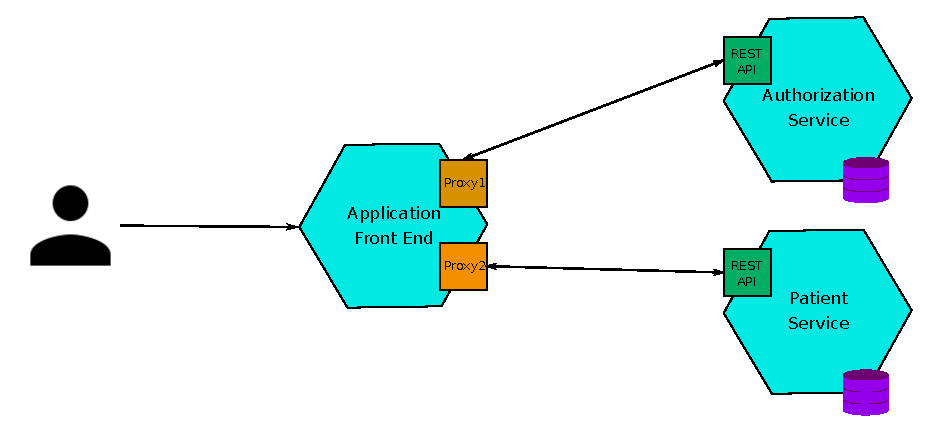
\includegraphics[width=0.45\textwidth]{./figs/mrs-mics2.eps}}
	\caption{An Example MRS.}
	\label{fig:mrs-mics}
\end{figure}

However, the aforementioned policy entails to log all such accesses indefinitely. In reality, breaking the glass is deactivated once the critical situation is resolved. Therefore, we may consider some dual capability ``mend-the-glass'' that restores access control and enforces it fully, if the glass is already broken. Having this capability, the example break-the-glass policy can be restated as follows: \emph{``Store in the log all accesses to patient medical history by a user who has already broken the glass and has not mended it afterwards''.}  This updated more realistic specification goes beyond Horn clauses in expressivity.

Therefore, a compelling next step is to consider a more powerful instrumentation tool to implement logging specifications that support extended preconditions like the one discussed above. Our instrumentation tool relies on models of correct audit logging which support more expressive classes of logging specifications.



%paper outline

\textbf{\textit{Paper outline.}}
The rest of the paper is organized as follows. In Section \ref{sec:implmodel}, we review the formal implementation model, discussing an instrumentation algorithm for systems in $\pi$-calculus. In Section \ref{sec:impl}, we discuss our tool to instrument microservices in Java Spring. In addition, we present a demo of a microservices-based MRS, and its instrumentation by our tool. 
%Section \ref{sec:eval} provides an empirical analysis of the instrumented applications, focusing on runtime overhead. 
%In Section \ref{sec:discussion}, we describe the limitations of this work, and potential future work. 
%Related work is discussed in Section \ref{sec:relwork}. Finally, Section \ref{sec:conclusion} concludes the paper.
Section \ref{sec:rwc} disucsses the related work and concludes the paper.

\section{A Brief Review of the Instrumentation Model} \label{sec:implmodel}

In \cite{X}, we have explored the full formalization of the implementation model for instrumenting concurrent systems that guarantee the correctness of audit logs, according to logging specifications that go beyond Horn clauses. In this section, we review this model briefly. 

\subsection{Source System Model} \label{sec:pi}

The source system $\srclang$ is concurrent program, which is modeled in $\pi$-calculus \cite{parrow2001introduction}. Top-level components of $\srclang$, denoted by $A$, are called top-level agents. Top-level agents execute in parallel, and communicate among themselves as their functionality dictates. Some $A$ consists of internal modules and/or functions, modeled as subagents $B^A$. As part of the definition of the source system, we assume the existence of a codebases $\codebaseu$ and $\codebasel$ that include definitions of the form $A(x_1, \cdots, x_n) \triangleq \cdots$ and $B^A (x_1, \cdots, x_n) \triangleq \cdots$ resp.



\subsection{A Class of Logging Specifications} \label{sec:logspec}
Horn clause logic has been used to specify audit logging requirements in previous work \cite{X}, where certain events must take place so that audit logs are generated. In this paper, we go beyond Horn clauses in our implementation model to help specify not only the necessity of having certain events to occur, but also to ensure that another group of events do not take place. In this respect, we define a class of specifications that assert temporal relations among the events that must or must not transpire in different components (top-level agents) of the system. Using this extended class of specifications, a particular event must be logged, provided that a certain set of events have taken place and another set of events have not. We would call these different sets of events positive and negative triggers, resp. We use $\callpols$ to denote this class of specifications. In $\callpols$, each event is modeled as a sub-agent invocation, i.e., a module within one of the agents of the system. Figure \ref{fig:callpols} depicts the structure of specifications in $\callpols$. $\folp{Call}(t,A,B,mathit{xs})$ asserts the event of invoking sub-agent $B^A$ at time $t$ with list of parameters $\mathit{xs}$. $\phi$ and $\psi_j$ are possibly empty conjunctive sequence of literals of the form $t_i < t_j$. $A_0$ is called a \emph{logging event agent}, whereas other $A_i$s are called \emph{positive trigger agents}. $A'_j$s are called \emph{negative trigger agents}. Similarly, \emph{logging event sub-agent} refers to $B_0$, and other $B_i$s are called \emph{positive trigger sub-agents}. $B'_j$s are called \emph{negative trigger sub-agents}. \emph{Logging preconditions} are predicates $\folp{Call}(t_i,A_i,B_i,\tilde{x})$ for all $i \in \{1,\cdots, n\}$ and $\folp{Call}(t_j , A'_j , B'_j , \mathit{ys}_j )$ for all $j \in \{1, \cdots, m\}$. 

For example, in the microservices-based MRS, described in Figure \ref{X}, each microservice, including Authorization and Patient, is a top-level agent in $\srclang$. Authorization may include modules to break and mend the glass, and Patient may have a functionality to read patient medical history. These functionalities are defined as part of $\codebasel$ (Figure \ref{X}). Moreover, Figure \ref{X} describes the logging specification in $\callpols$ that is associated with the break-the-glass policy. In this clause, $t_0$ and $t_1$ are timestamps, and $t_1$ precedes $t_0$. $p$ refers to the patient identifier, and $u$ is the user identifier who breaks the glass and attempts to read the medical history of p later on. Additionally, logging is preconditioned on the fact that the glass is not mended in between the events of breaking the glass and gaining access to the patient medical data. 


\begin{figure}
\setlength{\fboxsep}{0pt}%%%%%%%%
\fbox{\tiny{
\begin{mathpar}
\forall t_0, \cdots, t_n, \mathit{xs_0}, \cdots, \mathit{xs_n} \, . \, 
\folp{Call}(t_0,A_0,B_0,\mathit{xs_0}) \bigwedge_{i=1}^{n} \big(\folp{Call}(t_i,A_i,B_i,\mathit{xs_i}) \wedge t_i < t_0 \big) \wedge \varphi(t_0, \cdots, t_n) \wedge \varphi'(\mathit{xs_0}, \cdots, \mathit{xs_n}) 
\bigwedge_{j=1}^{m} \big( \forall t'_j, \mathit{ys}_j \, . \, \psi_j(\mathit{xs}_0, \cdots, \mathit{xs}_n, \mathit{ys}_j) \wedge \psi'_j(t_0, \cdots, t_n, t'_j) \implies \neg \folp{Call}(t'_j, A'_j, B'_j, \mathit{ys}_j) \big) 
 \implies \folp{LoggedCall}(A_0,B_0,\mathit{xs_0})
\end{mathpar}
}}
\caption{$\callpols$ clause structure.} 
\label{fig:callpols}
\end{figure}


\begin{figure}
\setlength{\fboxsep}{0pt}%%%%%%%%
\fbox{\tiny{
\begin{mathpar}
\codebasel(\mathtt{Authorization})(\mathtt{breakTheGlass}) = [\mathtt{breakTheGlass}^{\mathtt{Authorization}} \triangleq P] \mbox{~for~some~} P 

\codebasel(\mathtt{Patient})(\mathtt{getMedicalHistory}) = [\mathtt{getMedicalHistory}^{\mathtt{Patient}} \triangleq Q] \mbox{~for~some~} Q  


\forall t_0, t_1, p, u \, . \, \folp{Call}(t_0,\mathtt{Patient}, \mathtt{getMedicalHistory},[p,u]) \wedge \folp{Call}(t_1,\mathtt{Authorization}, \mathtt{breakTheGlass},[u]) \wedge t_1 < t_0 \implies \folp{LoggedCall}(\mathtt{Patient}, \mathtt{getMedicalHistory},[p,u])

\end{mathpar}
}}
\caption{Example logging specification for an MRS.}
\label{fig:exm-logspec}
\end{figure}

\subsection{Target System Model} \label{sec:pi-log}
The instrumentation algorithm maps a $\srclang$ system to a target system, denoted by $\trglang$ system. Runtime environment of $\trglang$ includes a timing counter $t$, $\locprec$ that returns the set of logging preconditions transpired in a given agent, $\remprec$ that returns the set of logging preconditions that have transpired the triggers of a given agent, and $\logmap$ that stores the audit logs for a given agent. The preconditions in $\remprec$ must be communicated between a given agent and all triggers agents. Certain prefixes are added to $\trglang$ to facilitate storage and retrieval of information to these runtime components: 1) $\callev(A,B,\tilde{x})$ updates $\locprec(A)$ with predicate $\folp{Call}(t,A,B,\tilde{x})$, 2) $\addprecond(x,A)$ updates$\remprec(A)$ with precondition $x$, 3) $\sendprecond(x,A)$ converts $\locprec(A)$ to a transferable object and sends it though link $x$, and 4) $\emitev(A,B,\tilde{x})$ studies the derivability of $\folp{LoggedCall}(A,B,\tilde{x})$ and accordingly $\logmap(A)$ is updated with this predicate. 


\subsection{Instrumentation Algorithm} \label{sec:inst-alg}
Instrumentation algorithm $\rewrite$ takes a $\srclang$ system and a logging specification from $\callpols$, and produces a $\trglang$ system with the following details. $\rewrite$ adds fresh links $c_{ij}$ between every logging event agent $A_i$ and trigger agent $A_j$, in order to communicate logging preconditions (by $\sendprecond$ and $\addprecond$ prefixes). If sub-agent $B^A$ is a trigger, then its execution must be preceded by $\callev$ prefix, so that the logging precondition is stored in $\locprec(A)$. If sub-agent $B^A$ is a logging event agent, the execution of $B^A$ must be preceded by $\callev$, similar to the previous case. Next, it must communicate on appropriate links ($c_{ij}$s) with all trigger agents. To this end, $B^A$ is supposed to notify each of those agents to send their collected preconditions, and then it must add them to $\remprec(A)$. This is done using $\addprecond$ prefixes. Then, it should study whether the invocation needs to be logged, before following normal execution. This is facilitated by $\emitev$ prefix. 

If $A_j$ is a trigger agent then it must be able to handle incoming requests for collected preconditions. This is done by adding a fresh sub-agent to $A_j$ that always listens for requests on the dedicated link ($c_{ij}$) between itself and the logging event agent. This sub-agent is denoted by $D_{ij}$. Upon receiving such a request, $D_{ij}$ sends back the preconditions, handled by prefix $\sendprecond$, and then continues to listen on $c_{ij}$.

As an example consider the instrumentation of the MRS described in Figures \ref{fig:mrs-mics} and \ref{fig:exm-logspec}. According to the logging specification, $\mathtt{getMedicalHistory}^{\mathtt{Patient}}$ is the logging event, and $\mathtt{breakTheGlass}^{\mathtt{Authorization}}$ is the only trigger. $\rewrite$ instruments the system as described in Figure \ref{fig:exm-inst}.  A new link $c_{\mathtt{PA}}$ is established between the two agents, and sub-agents are instrumented accordingly. In addition, sub-agent $D_{\mathtt{PA}}$ is added to $\mathtt{Authorization}$ microservice that indefinitely responds to the requests from $\mathtt{Patient}$ microservice on $c_{\mathtt{PA}}$.

\begin{figure}
\setlength{\fboxsep}{0pt}%%%%%%%%
\fbox{\tiny{
\begin{mathpar}
\codebasel'(\mathtt{Authorization})(\mathtt{breakTheGlass}) = \big[\mathtt{breakTheGlass}^{\mathtt{Authorization}}(u) \triangleq \callev(\mathtt{Authorization},\mathtt{breakTheGlass},[u]).P \big]

\codebasel'(\mathtt{Patient})(\mathtt{getMedicalHistory}) = \big[ \mathtt{getMedicalHistory}^{\mathtt{Patient}}(p,u) \triangleq \callev(\mathtt{Patient},\mathtt{getMedicalHistory},[p,u]).\outprefix{c_{\mathtt{PA}}}{}.c_{\mathtt{PA}}(f). \addprecond(f,\mathtt{Patient}). \newline \emitev(\mathtt{Patient},\mathtt{getMedicalHistory},[p,u]).Q \big]


\codebasel'(\mathtt{Authorization})(D_{\mathtt{PA}}) =  \big[ D{_{\mathtt{PA}}^{\mathtt{Authorization}}}(c_{\mathtt{PA}}) \triangleq 
c_{\mathtt{PA}}.\sendprecond(c_{\mathtt{PA}},\mathtt{Authorization}). D{_{\mathtt{PA}}^{\mathtt{Authorization}}}(c_{\mathtt{PA}}) \big]

\end{mathpar}
}}
\caption{Example Instrumentation of the MRS.}
\label{fig:exm-inst}
\end{figure}

 %implementation model

\section{Instrumenting Microservices} \label{sec:impl}
In this section, we explain the implementation of the instrumentation algorithm for microservices-based applications, as well as a demo of how the tool modifies these applications based on different logging specifications. In our instrumentation tool, each microservice of an application is treated as an agent of the concurrent system, whereas each method defined in some library of a microservice is considered as a sub-agent.% of that agent.

\subsection{Instrumentation Tool: $\tool$} \label{sec:impl-tool}
We have implemented the proposed algorithm $\rewrite$ for microservices-based applications that are deployed using Java Spring Framework. % \cite{johnson2004spring}. 
Our instrumentation tool \cite{github1}, 
$\tool$, receives a logging specification along with an application consisting of two or more microservices, and rewrites those microservices accordingly. $\tool$ extends microservices with required RESTful APIs that facilitate the communication between microservices for the sake of audit logging. %$\tool$ receives three arguments described in the following.

The logical specification of logging requirements (Section \ref{sec:logspec}) is passed as an argument to $\tool$ in JSON format. $\tool$ parses this JSON file and extracts logging specification in the form of Horn clauses, along with identifying triggers and logging events.
The paths to different microservices of the application are also passed to $\tool$. %For this purpose, $\tool$ expects a file with paths to different microservices. These microservices are supposed to be built by Java Spring Framework. 
$\tool$ applies modifications to each microservice component according to the logging specification.
In addtion, the path to the Prolog engine must be fed to $\tool$. $\tool$ uses SWI Prolog \cite{swi} to logically infer the derivation of logging events according to the logging specification, the set of facts regarding trigger events, etc.% as well as any other collection of facts that are potentially needed\footnote{Note that there could be preconditions beyond trigger events.}.

%\begin{itemize}
%	\item The logical specification of logging requirements (Section \ref{sec:logspec}) is passed as an argument to $\tool$ in JSON format. $\tool$ parses this JSON file and extracts logging specification in the form of Horn clauses, along with identifying triggers and logging events.
%	\item The microservices-based application is passed as another argument to $\tool$. For this purpose, $\tool$ receives a text file with paths to different microservices. These microservices are supposed to be built by Java Spring Framework. $\tool$ applies modifications to each microservice component according to the logging specification.
%	\item The last argument to $\tool$ is the path to the Prolog engine in the local system. $\tool$ uses SWI Prolog \cite{swi} to logically infer the derivation of logging events according to the logging specification, the set of facts regarding trigger events, as well as any other collection of facts that are potentially needed\footnote{Note that there could be arbitrary preconditions in the logging specification that may require gathering facts beyond trigger events.}.
%\end{itemize}

$\tool$ uses aspect-oriented programming (AOP), in particular AspectJ, %\cite{laddad2009aspectj}, 
to weave concurrent logging capability into microservices. For this purpose, $\tool$ extends the Project Object Model of the microservices which need to be instrumented by \texttt{spring-boot-starter-aop} dependency. 
%(Figure \ref{fig:aop-dep}).
%
%\begin{figure}
%\begin{scriptsize}
%\begin{Verbatim}[frame=single]
%...
%<dependency>
%  <groupId>org.springframework.boot</groupId>
%  <artifactId>spring-boot-starter-aop</artifactId>
%</dependency>
%...
%\end{Verbatim}
%\end{scriptsize}
%\caption{AOP dependency.}
%\label{fig:aop-dep}
%\end{figure}

According to the implementation model, the configuration of the concurrent system includes three different structures to store the logging preconditions that are transpired locally ($\locprec$), logging preconditions that are originated remotely ($\remprec$), and the audit logs recorded by an agent ($\logmap$). These structures are added by $\tool$ as repositories of logical facts that are kept on nonvolatile memory. If a microservice is only a trigger, then a repository is added to that microservice to store logging preconditions that take place locally in that microservice. However, if a microservice is a logging event, then that microservices is extended with all three types of repositories. 
%to store locally and remotely transpired preconditions, as well as the audit logs. 
We call these repositories \texttt{local-db}, \texttt{remote-db}, and \texttt{log-db}, resp. Note that according to the definition of $\rewrite$ (Section \ref{sec:inst-alg}), a trigger is only concerned with locally transpired preconditions (through $\callev$ prefixes), whereas a logging event needs to access all three types of aforementioned structures (through $\callev$, $\addprecond$, and $\emitev$ prefixes).

$\rewrite$ extends every trigger with sub-agents, $D_{ij}$, that send back the locally generated preconditions upon receiving a request on a dedicated link (using $\sendprecond$ prefix). $\tool$ implements this feature by extending each trigger microservice with a REST controller that sends back the content of \texttt{local-db}, if it receives an HTTP GET request on the dedicated path \texttt{/localdb}. This controller is denoted by \texttt{LocalDBController}, henceforth. On the other side, a logging event microservice is supposed to contact the trigger on dedicated links to receive the preconditions that are transpired in trigger agents. $\tool$ facilitates this by extending every logging event microservice with a web client that sends asynchronous HTTP GET requests to \texttt{/localdb} path on trigger microservices and collects the responses. We have called this service \texttt{RestClient}.

As mentioned earlier, AOP is used to add logging capabilities to microservices. For this purpose, $\tool$ identifies the pointcuts in which an advice needs to be defined. According to $\rewrite$, trigger sub-agents are preceded by $\callev$ prefixes. For this purpose, $\tool$ defines \textit{before} aspects for each of the trigger methods, where the advice includes the construction of preconditions from the join points and adding them to \texttt{local-db}. This implements the semantics of $\callev$.%, given in Figure \ref{fig:before-asp}.

$\rewrite$ instruments logging event sub-agents by inserting a sequence of operations before the execution of these sub-agents. This sequence includes $\callev$ prefixes, communication on dedicated links to receive remotely transpired logging preconditions, adding them to $\remprec$ using $\addprecond$ prefixes, and finally checking if logging events should to be logged, using $\emitev$. $\tool$ handles this by defining \textit{before} aspects for the pointcuts that correspond to logging event methods. Similar to the aspects defined for trigger methods, the advice for logging event methods starts with the construction of preconditions from join points and adding them to \texttt{local-db}. Next, \texttt{RestClient} is used to asynchronously send an HTTP GET request on the predefined path \texttt{/localdb} to each of the trigger microservices, and collect the results in \texttt{remote-db}. This implements the semantics of $\addprecond$ prefix. Then, SWI Prolog engine is invoked to add the logging specification, and the contents of \texttt{local-db} and \texttt{remote-db}. Finally, the Prolog engine is queried to study if the invocation of logging event must be logged, and accordingly \texttt{log-db} repository is updated. These final steps implement the semantics of $\emitev$ prefix. In order to facilitate the communication between SWI Prolog engine and Java Virtual Machine, InterProlog Java/Prolog SDK \cite{calejo2004interprolog} is used. 

Figure \ref{fig:before-asp} specifies the advice for triggers and logging events in general form. Figure \ref{fig:log-inst} depicts some of the aforementioned modifications that $\tool$ applies architecturally to the logging event and trigger microservices.

\begin{figure}
\begin{tiny}
\begin{Verbatim}[frame=single]
@Before("execution (some trigger)")
public void someAspect(JoinPoint){
	...
	build precondition from JoinPoint
	add precondition to local-db
	...
}

@Before("execution (some logging event)")
public void someAspect(JoinPoint) {
	...
	build precondition from JoinPoint
	add precondition to local-db
	...
	send GET to triggers
	collect the responses in remote-db
	...
	add logging specification to the engine
	add the content of local-db to the engine
	add the content of remote-db to the engine
	query the engine and update log-db
	...	
}
\end{Verbatim}
\end{tiny}
\caption{Pseudocode of \textit{before} advice for triggers and logging events.}
\label{fig:before-asp}
\end{figure}


%\begin{figure}
%\begin{scriptsize}
%\begin{Verbatim}[frame=single]
%
%\end{Verbatim}
%\end{scriptsize}
%\caption{Pseudocode of \textit{before} advice for logging events.}
%\label{fig:before-asp-logev}
%\end{figure}


%\subsection{A Demo of Microservices-based Medical Records Systems} \label{sec:impl-demo}
\subsection{Case Study: Instrumenting $\demo$ with $\tool$} \label{sec:cstudy}
In Section \ref{sec:intro}, we discussed an oversimplified MRS consisting of several loosely-coupled microservices. We have implemented \cite{github2} 
a demo of this system, $\demo$, consisting of several microservices, using Java Spring Boot \cite{webb2013spring}. The front-end microservice of $\demo$ authenticates users and acts as the API gateway by relaying requests to the back-end microservices. %$\demo$ consists of the following microservices.

%\paragraph{\texttt{authorization-service}} 
%\textbf{\texttt{authorization-service.}}
%This microservice provides different functionalities regarding user access to system resources. The main component of this microservice is a REST controller that provides API to check access status of some user to a system resource, break the glass by some user, check if the glass is broken for some user, and retrieve the list of users who have currently broken the glass.

%\paragraph{\texttt{patient-service}} 
%\textbf{\texttt{patient-service.}}
%This microservice implements patient data model, which includes patient ID, name, and patient disease. Patient microservice uses Java Persistent API (JPA) to map patient data model to a relational database entity. It includes an extension to JPA repository interface that manages access to the patient entity. Patient microservice uses a relational database for this purpose. %\cite{h2db} swhich is populated by a SQL file from disk at the startup.
%\footnote{Indeed, in a more realistic setting, a database management system with nonvolatile storage must be used.}. 
%Patient microservice includes a REST controller that provides API to read patient information from the database using JPA repository interface. The API includes retrieving 1) patient medical history by ID and patient name, 2) all patients with a certain disease, and 3) the information of all patients.


%\begin{figure} [h]
%	\centering
%	\fbox{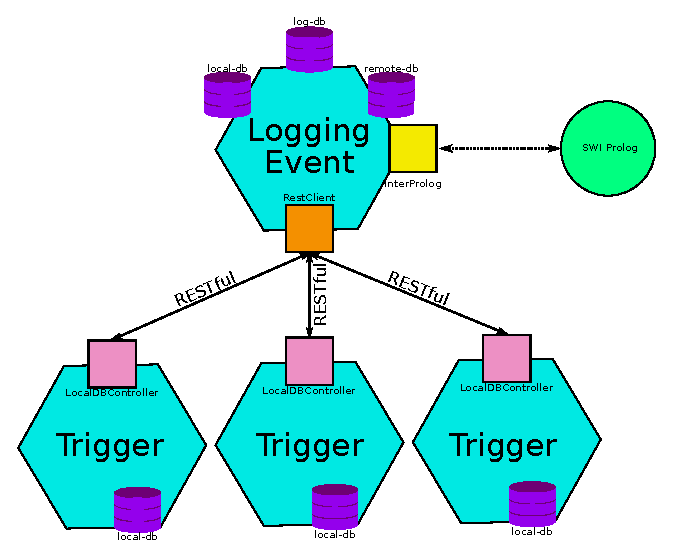
\includegraphics[width=0.45\textwidth]{./figs/log-inst.eps}}
%	\caption{Structure of the logging event and trigger microservices, instrumented by $\tool$.}
%	\label{fig:log-inst}
%\end{figure}

%\paragraph{\texttt{authentication-service}} 
%\textbf{\texttt{authentication-service.}}
%This microservice implements the application front-end as a web user interface through a collection of Java Server Pages, as well as two proxies that provide APIs to communicate with the two other microservices. The application front-end uses a login service that mimics the authentication of users based on their credentials. Authentication microservice defines REST controllers that employ OpenFeign proxies to relay user requests (coming from web UI) to Patient and Authorization microservices.

%\begin{itemize}
%	\item Authorization Microservice (\texttt{authorization-service}): This microservice provides different functionalities regarding user access to system resources. The main component of this microservice is a REST controller that provides API to check access status of some user to a system resource, break the glass by some user, check if the glass is broken for some user, and retrieve the list of users who have currently broken the glass.
%%	\begin{itemize}
%%		\item check access status of some user to a system resource,
%%		\item break the glass by some user,
%%		%\item mend the glass by some user,
%%		\item check if the glass is broken for some user, and
%%		\item retrieve the list of users who have currently broken the glass.
%%	\end{itemize}
%	
%	\item Patient Microservice (\texttt{patient-service}): This microservice implements patient data model, which includes patient ID, name, and patient disease. Patient microservice uses Java Persistent API (JPA) to map patient data model to a relational database entity. It includes an extension to JPA repository interface that manages access to the patient entity. Patient microservice uses H2 in-memory database \cite{h2db} which is populated by a SQL file from disk at the startup\footnote{Indeed, in a more realistic setting, a database management system with nonvolatile storage must be used.}. Patient microsevice includes a REST controller that provides API to read patient information from H2 database using JPA repository interface. The API includes retrieving patient medical history by ID, retrieving patient medical history by name, retrieving all patients with a certain disease, and retrieving the information of all patients.
%%	\begin{itemize}
%%		\item retrieving patient medical history by ID,
%%		\item retrieving patient medical history by name,
%%		\item retrieving all patients with a certain disease, and
%%		\item retrieving the information of all patients.
%%	\end{itemize}
%	
%	\item Authentication Microservice (\texttt{authentication-service}): This microservice implements the application front-end as a web user interface through a collection of Java Server Pages, as well as two Feign proxies that provide APIs to communicate with the Authorization and Patient microservices. The application front-end uses a login service that mimics the authentication of users based on their credentials. Authentication microservice defines REST controllers that employ OpenFeign proxies to relay user requests (coming from web UI) to Patient and Authorization microservices.
%\end{itemize}
%Figure \ref{fig:mrs-mics-impl} demonstrates the high-level architecture $\demo$.

%Figure \ref{fig:mrs-mics} depicts the high-level structure of $\demo$, where the application front-end is the Authentication microservice.

%\begin{figure} 
%	\centering
%	\fbox{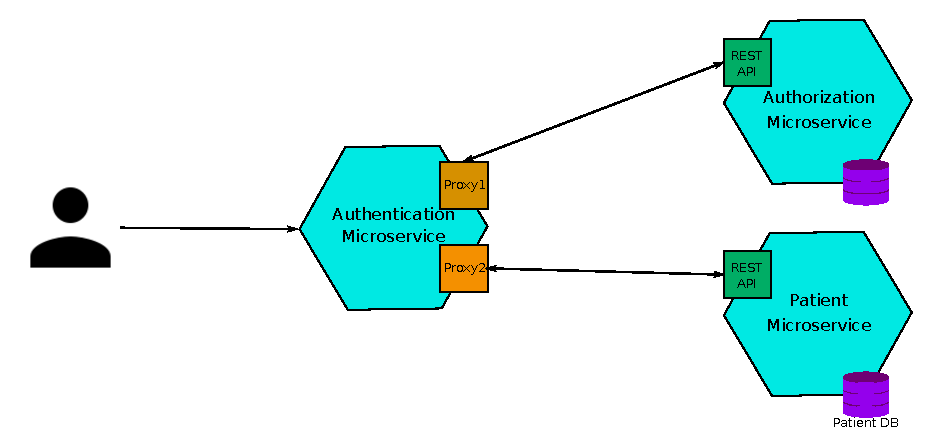
\includegraphics[width=0.45\textwidth]{./figs/mrs-mics3.eps}}
%	\caption{High-level architecture of $\demo$.}
%	\label{fig:mrs-mics-impl}
%\end{figure}

%\subsection{Case Study: Instrumenting $\demo$ with $\tool$} \label{sec:cstudy}
%As mentioned in Section \ref{sec:impl-tool}, $\tool$ receives the logging specification in JSON format, along with the different microservices of a system that may need to be instrumented. As a case study, 
In the following, we explain how $\demo$ is instrumented by $\tool$ for a given logging specification. In Figure \ref{fig:exm-logspec}, we have described a logging specification that enforces logging access to patient medical history at any point after breaking the glass. We can assert a similar logging specification rule in JSON \cite{github1}
, which is more verbose than its logical equivalent. $\tool$ parses that JSON specification and constructs the Horn clause given in Figure \ref{fig:brk-horn} (ver. 1), which is then added to SWI Prolog engine fact base.
Note that in this Horn clause presentation, we have redacted the full package names of the trigger and logging event methods and replaced them with \texttt{<package>}, for the sake of space economy.  $\tool$ instruments $\demo$ according to this logging specification rule as follows: \texttt{spring-boot-starter-aop} dependency is added to the POM of Patient and Authorization services. Authorization service is extended with  \texttt{local-db}.  Patient service is extended with \texttt{local-db}, as well as \texttt{remote-db}, and \texttt{log-db}. Authorization service is extended with the REST controller \texttt{LocalDBController} that responds to requests on path \texttt{/localdb}.  Patient service is extended with \texttt{RestClient} web client. A \textit{before} aspect is added to Authorization service with \texttt{AuthorizationController.breakTheGlass} as its pointcut. This aspect builds preconditions from the join point and appends them to \texttt{local-db}. A \textit{before} aspect is added to Patient service with pointcut \texttt{PatientController.getPatientMedHistByName}, to 1) build preconditions from the join point and append them to \texttt{local-db}, 2) send HTTP GET request on path \texttt{/localdb} to Authorization service, and store the results in \texttt{remote-db} repository,  3) add the logging specification, and contents of \texttt{local-db} and \texttt{remote-db} repositories to the SWI Prolog engine, and 4) send queries to the Prolog engine to check derivability of \texttt{loggedfunccall} predicates and accordingly update \texttt{log-db} with the engine's response.
 
%1) \texttt{spring-boot-starter-aop} is added as a dependency to the POM of both \texttt{patient-service} and \texttt{authorization-service}. 2) \texttt{local-db} repository is added to  \texttt{authorization-service}. 3) \texttt{local-db}, \texttt{remote-db}, and \texttt{log-db} repositories are added to \texttt{patient-service}. 4) \texttt{LocalDBController} is added to  \texttt{authorization-service} to respond to requests on path \texttt{/localdb}. 5) \texttt{patient-service} is extended with \texttt{RestClient} web client service. 6) A \textit{before} aspect is added to \texttt{authorization-service} with \texttt{AuthorizationController.breakTheGlass} as its pointcut. This aspect builds preconditions from the join point and appends them to \texttt{local-db}. 7) A \textit{before} aspect is added to \texttt{patient-service} with \texttt{PatientController.getPatientMedHistByName} as its pointcut. This aspect i) builds preconditions from the join point and appends them to \texttt{local-db}, ii) sends HTTP GET request to \texttt{authorization-service} on path \texttt{/localdb}, and stores the results in \texttt{remote-db} repository,  iii) adds the logging specification, and contents of \texttt{local-db} and \texttt{remote-db} repositories to the SWI Prolog engine, and iv) sends queries to the Prolog engine to check derivability of \texttt{loggedfunccall} predicates and accordingly updates \texttt{log-db} with the engine's response.


\begin{figure}
\begin{tiny}
\begin{Verbatim}[frame=single]
/* Version 1 */
loggedfunccall(T0, patient-service, 
  "<package>.PatientController.getPatientMedHistByName", [U, P]) :-
 funccall(T0, patient-service, 
  "<package>.PatientController.getPatientMedHistByName", [U, P]), 
 funccall(T1, authorization-service, 
  "<package>.AuthorizationController.breakTheGlass", [U]), 
 <(T1, T0), ==(U, user).
 
/* Version 2 */
loggedfunccall(T0, patient-service, 
  "<package>.PatientController.getPatientMedHistByName", [U, P]) :-
 funccall(T0, patient-service, 
  "<package>.PatientController.getPatientMedHistByName", [U, P]), 
 funccall(T1, authorization-service, 
  "<package>.AuthorizationController.breakTheGlass", [U]), 
 funccall(T2, authentication-service, 
  "<package>.AuthenticationService.authenticate", [U]), 
 <(T1, T0), <(T2, T1), ==(U, user).
 
/* Version 3 */
loggedfunccall(T0, patient-service, 
  "<package>.PatientController.getPatientMedHistByName", [U, P]) :- 
 funccall(T0, patient-service, 
  "<package>.PatientController.getPatientMedHistByName", [U, P]), 
 funccall(T1, authorization-service, 
  "<package>.AuthorizationController.breakTheGlass", [U]), 
 funccall(T2, patient-service, 
  "<package>.PatientController.getAllPatients", [U]),
 funccall(T3, authorization-service, 
  "<package>.AuthorizationController.getBTGUsers", []), 
  <(T1, T0), <(T2, T0), <(T3, T0), ==(U, user).
\end{Verbatim}
\end{tiny}
\caption{Different versions of break-the-glass policy specified as a Horn clause.}
\label{fig:brk-horn}
\end{figure}




%\begin{itemize}[leftmargin=*]
%	\item \texttt{spring-boot-starter-aop} dependency is added to the POM of \texttt{patient-service} and \texttt{authorization-service}.
%	
%	\item \texttt{authorization-service} is extended with  \texttt{local-db}.% repository.
%
%	\item \texttt{patient-service} is extended with \texttt{local-db}, as well as \texttt{remote-db}, and \texttt{log-db}.% repositories.
%
%	\item \texttt{authorization-service} is extended with the REST controller \texttt{LocalDBController} that responds to requests on path \texttt{/localdb}.
%
%	\item \texttt{patient-service} is extended with \texttt{RestClient} web client. 
%
%	\item A \textit{before} aspect is added to \texttt{authorization-service} with \texttt{AuthorizationController.breakTheGlass} as its pointcut. This aspect builds preconditions from the join point and appends them to \texttt{local-db}.
%	
%	\item A \textit{before} aspect is added to \texttt{patient-service} with pointcut \texttt{PatientController.getPatientMedHistByName}, to 1) build preconditions from the join point and append them to \texttt{local-db}, 2) send HTTP GET request on path \texttt{/localdb} to \texttt{authorization-service}, and store the results in \texttt{remote-db} repository,  3) add the logging specification, and contents of \texttt{local-db} and \texttt{remote-db} repositories to the SWI Prolog engine, and 4) send queries to the Prolog engine to check derivability of \texttt{loggedfunccall} predicates and accordingly update \texttt{log-db} with the engine's response.
%\end{itemize}
These changes describe the real-world instrumentation of the MRS, formally given in Figure \ref{fig:exm-inst}.
Note that Authentication microservice is unaffected when instrumented by $\tool$, as it does not include any trigger or logging event methods according to the logging specification.

%\begin{figure} 
%	\centering
%	\fbox{\includegraphics[width=0.45\textwidth]{./figs/mrs-mics-target.eps}}
%	\caption{High-level architecture of $\demo$ after instrumentation by $\tool$ using the specification of Figure \ref{fig:brk-horn}.}
%	\label{fig:mrs-mics-target}
%\end{figure}

The two other versions (Figure \ref{fig:brk-horn}) are example extensions to the policy ver. 1 . In ver. 2, authenication is considered as an additional trigger. Therefore, in addition to the aforementioned changes, $\tool$ extends Authentication microservice with  \texttt{local-db} repository, \texttt{LocalDBController}, and a \textit{before} aspect (trigger version). The \textit{before} aspect of Patient microservice is also extended with sending HTTP GET requests to Authentication microservice on path \texttt{/localdb}, and storing the results in \texttt{remote-db}. In ver. 3, two additional triggers are considered in Authorization and Patient microservices. $\tool$ applies the same changes given above, along with defining \textit{before} aspects for each extra trigger. Figures \ref{fig:mrs-mics-target} and \ref{fig:mrs-mics-target2} visually describe some of the aforementioned changes to $\demo$ by $\tool$, considering each version of the policy.%\footnote{For the sake of anonymity, we have avoided to cite the associated Github repository that includes $\tool$, $\demo$, several JSON specifications of the logging requirements and the associated instrumented versions of $\demo$. However, these implementation details can be provided by the authors if requested for reviewing purposes.}. 
These instrumented versions are accessible in \cite{github1}, along with other examples of logging specifications, and their associated instrumented counterparts.

	\begin{figure*}
        \centering
        \begin{subfigure}[b]{0.31\textwidth}
            \centering
            \fbox{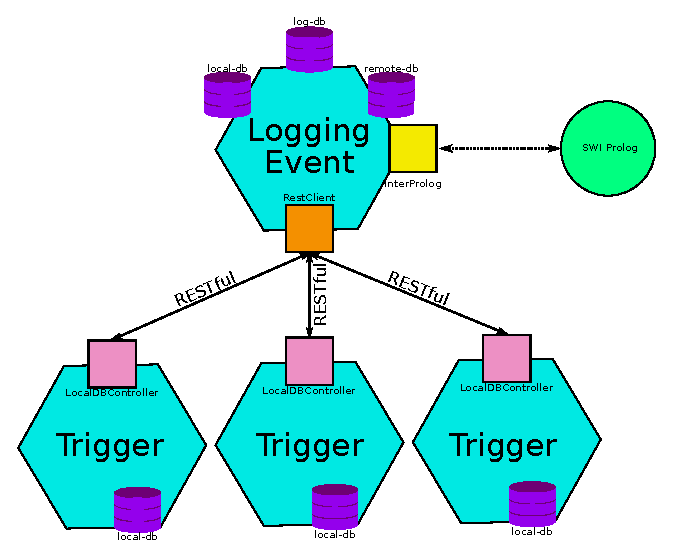
\includegraphics[width=\textwidth]{./figs/log-inst.eps}}
            \caption[]%
            {{\small Structure of the logging event and trigger microservices, instrumented by $\tool$.}}    
            \label{fig:log-inst}
        \end{subfigure}
        \hfill
        \begin{subfigure}[b]{0.32\textwidth}   
            \centering 
            \fbox{\includegraphics[width=\textwidth]{./figs/mrs-mics-target.eps}}
             \caption[]%
            {{\small $\demo$ instrumented by $\tool$ using versions 1 and 3 in Figure \ref{fig:brk-horn}.}}    
            \label{fig:mrs-mics-target}
        \end{subfigure}
        \hfill
        \begin{subfigure}[b]{0.32\textwidth}   
            \centering 
            \fbox{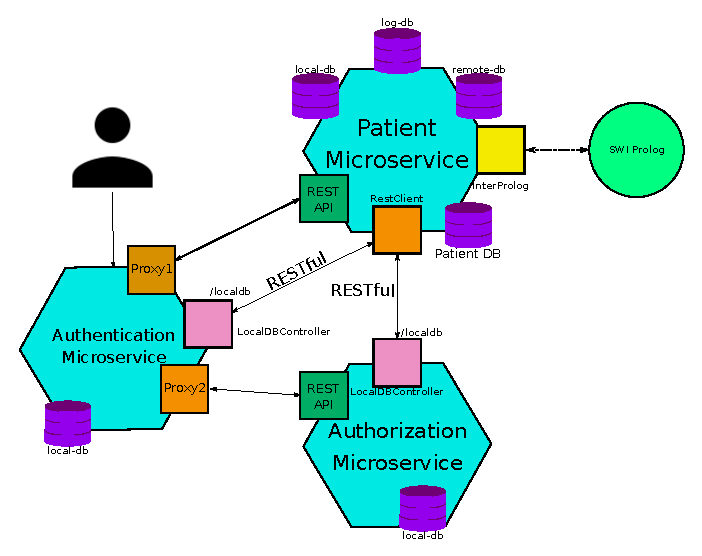
\includegraphics[width=\textwidth]{./figs/mrs-mics-target2.eps}}
            \caption[]%
            {{\small $\demo$ instrumented by $\tool$ using version 2 in Figure \ref{fig:brk-horn}.}}    
            \label{fig:mrs-mics-target2}
        \end{subfigure}
        \vspace{5mm}
        \caption[]
        {\small Architecture of microservices after instrumentation.} 
       \label{fig:mrs-structure}
    \end{figure*}

%\begin{figure} 
%	\centering
%	\fbox{\includegraphics[width=0.45\textwidth]{./figs/mrs-mics-target.eps}}
%	\caption{High-level architecture of $\demo$ after instrumentation by $\tool$ using version 1 and 3 specifications of Figure \ref{fig:brk-horn}.}
%	\label{fig:mrs-mics-target}
%\end{figure}
%
%\begin{figure} 
%	\centering
%	\fbox{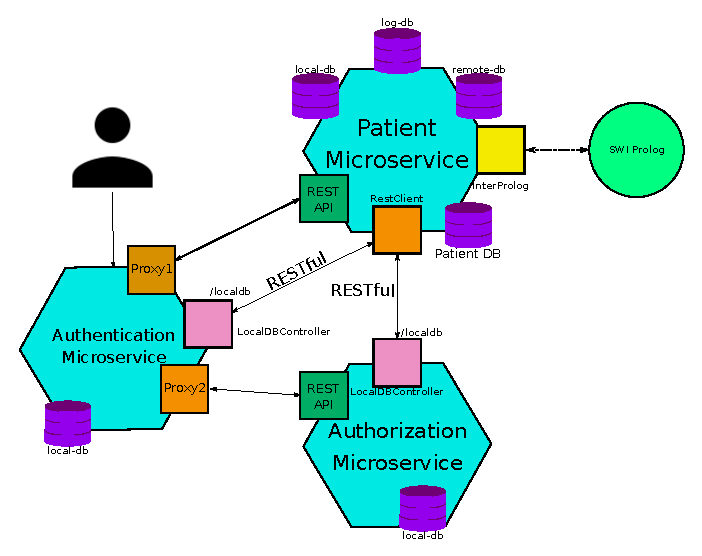
\includegraphics[width=0.45\textwidth]{./figs/mrs-mics-target2.eps}}
%	\caption{High-level architecture of $\demo$ after instrumentation by $\tool$ using version 2 specification of Figure \ref{fig:brk-horn}.}
%	\label{fig:mrs-mics-target2}
%\end{figure}

 %implementation

%\input{eval}

%\input{discussion} 

%\section{Related Work} \label{sec:relwork}

As microservices have gained more popularity in the application design and deployment in recent years, their safety and security have been the focus of several studies, e.g., \cite{mateus2021security, nkomo2019software, nehme2019securing, yu2019survey}. Most commonly in the realm of audit logging, a central approach has been considered, where a specific microservice is responsible to collect all logging events \cite{barabanov2021security, kazanavivcius2019migrating}. In particular, Elascale \cite{khazaei2017elascale} is a monitoring system that is deployed as an independent microservice. In contrast, Amir-Mohammadian et al. \cite{stpsa21} propose an instrumentation technique that enables concurrent audit logging in different microservices. $\tool$ \cite{github1} is the implementation of this instrumentation technique in the context of Java Spring microservices. Formal correctness of $\tool$ relies on information algebraic \cite{Kohlas14} semantics of audit logging, originally explored in \cite{lsfa20}  for concurrent systems. 

Operating system-level and network-level monitoring  has been a commonplace trend in audit logging for microservices. Examples include Amazon CloudeWatch \cite{cloudwatch}, Nagios \cite{nagios}, Microsoft Azure Kubernetes \cite{kuber}, and Spring Security Framework \cite{nguyen2019applying}. Cinque et al. \cite{cinque2019microservices} propose a blackbox tracing mechanism for monitoring microservices that does not involve instrumentation. 

In this paper, we propose a more powerful tool to support concurrent audit logging in microservices, whose formal correctness relies on an implementation model on concurrent systems \cite{amirmoh-tr21}.


%%\paragraph{Audit logging in microservices}
%\textbf{\textit{Audit logging in microservices.}}
%In recent years, constructing software in terms of decoupled microservices \cite{microservices, guidi2017microservices, soldani2018pains, salibindla2018microservices} has been a trending approach in web application design and deployment, and thus different studies have been conducted on microservices security \cite{micro-oreilly, nkomo2019software, nehme2019securing}. In practice, enforcing in-depth security has pushed platform-specific monitoring and logging techniques for microservices, e.g., in Azure Kubernetes Service \cite{kuber} and Spring Security Framework \cite{nguyen2019applying, baker2019novel}. One common approach has been to establish a central logging service with data visualization capabilities \cite{kazanavivcius2019migrating}. Examples include a  provenance logger for microservices-based applications \cite{curator}, and an architecture for IoT services that includes logger microservices in Web of Objects platform \cite{jarwar2017exploiting}.  Our approach in audit logging is concurrent rather than central, i.e., any microservice is able to log events based on preconditions that may occur in other microservices as well as that microservice. This boosts the expressivity of the enforcible logging policies. %2) We have a language-based approach to study audit logging with formal correctness guarantees, and then deploy it according to this language-based model. %Jolie \cite{jolie} is the dedicated programming language for microservices-based development of applications, whose semantics is heavily inspired by $\pi$-calculus \cite{guidi2006sock,montesi2011programming}. This has inspired us to study the correctness of audit logs for concurrent systems in this calculus rather than other language models. 
%There have been other approaches to define semantics of microservices, including Petri nets \cite{camilli2017formal}.
%
%
%%\paragraph{Formal study of audit logging}
%\textit{\textbf{Formal study of audit logging.}} 
%One line of work wrt formal study of audit logging focuses on the security of logs, in particular through cryptographic techniques, e.g., to establish forward secrecy \cite{Yavuz09}, to ensure trustworthiness of logs \cite{Bock:2010:TMT:1825731.1826135, Accorsi10}, and to preserve privacy in auditing \cite{Lee06}. These techniques assume that logs are given in the first place to be secured. However, in this paper we aim at developing a tool to generate audit logs according to a provably correct model, and thus security of the logged data is orthogonal to it. 
%
%Another line of work uses logical frameworks to establish accountability in access to system resources. Examples include a framework to enforce accountability goals in discretionary access control \cite{auditbased_compliance}, accountability wrt access to personal information based on owner-defined usage policies \cite{logic_audit}, distributed accountability based on turn-based games \cite{theorey_accountability}, and logging the proof of having access to system resources \cite{AURA, apple}. %Our logical framework for audit logging, however, does not limit it to a certain application, and can be used to instrument systems for different logging purposes.  
%Another related area of work is the language-level analysis of generated audit logs \cite{bavera2015justification,ricciotti2017strongly%,ricciotti2018explicit
%}. 
%
%%\paragraph{Correct audit logging} 
%\textit{\textbf{Correct audit logging.}}
%Information algebra \cite{Kohlas14} has been used to describe the semantics of audit logging \cite{amir-chong-skalka-post16} for linear process execution that defines notion of correctness for audit logs, along with an instrumentation model that guarantees to generate correct audit logs. %The same semantic framework has been used to enhance dynamic integrity information flow analysis through post-facto study of audit logs \cite{amir-skalka-plas16,jcs20} in a provable fashion. 
%Lately, an instrumentation model has been proposed for concurrent systems based on the information-algebraic semantic framework \cite{lsfa20}. This model enjoys correct audit logging, which has been the basis for our proposed instrumentation tool. %\cite{github1} 
%
%
%
%%\paragraph{Provenance} 
%\textit{\textbf{Provenance.}}
%Audit logging is closely associated with the notion of provenance tracking \cite{ricciotti2017core, herschel2017survey, buneman2019data}. Recent works in this area include ClearScope \cite{gordon2019precise} a provenance tracker for Android devices, CamFlow \cite{pasquier2017practical} an auditing and provenance capture utility in Linux, and AccessProv \cite{capobianco2017accessprov} an instrumentation tool to discover vulnerabilities in Java applications.


\section{Conclusion} \label{sec:conclusion}
In this paper, we have proposed an instrumentation tool for Java Spring based microservices to enforce audit requirements, whose logical specifications are not expressible by Horn clause logic. Our implementation tool is an extension of an earlier solution that supported specifications in Horn clauses. Our tool receives the specification in JSON format, along with the source code of microservices. It identifies the triggers and logging events in the application, and accordingly instruments them. As a case study, we discuss a microservices-based medical records system that lets users to deactivate controlling access to patient medical information in critical scenarios and activate it at a later stage. The correctness of the instrumentation tool relies on a formal model of the instrumentation that guarantees the generated logs to be necessary and sufficient.


%In this paper, we have proposed a tool, $\tool$, to instrument microservices-based applications that are deployed in Java Spring Framework for audit logging purposes. Our tool is based on an implementation model for concurrent systems that guarantees correctness of audit logging, using an information-algebraic semantic framework. $\tool$ receives the application source code, consisting of two or more microservices, along with a specification of audit logging requirements in JSON format. $\tool$ parses the JSON specification and extracts Horn clauses that are fed to a logic programming engine. $\tool$ instruments the microservices according to this specification. The instrumentation includes adding new repositories to the corresponding microservices, extending RESTful APIs on those microservices for logging-related communications, and weaving audit logging into the control flow of microservices using AspectJ. Our case study is a medical records system in which certain actions in authorization microservice may trigger logging events in access to patient medical data.




\bibliographystyle{IEEEtran}
\bibliography{bib}

%\appendix 
%\input{congr}


\end{document}

